\section{Signal Selection Strategy}
\label{sec:hh_strategy}

%%%%%%%%%%%%%%%%%%%%%%%%%%%%%%%%%%%%%%%%%%%%%%%%%%%%%%%%%%%%%%%%%%%%%%%%%%%%%%%%%%%
%%%%%%%%%%%%%%%%%%%%%%%%%%%%%%%%%%%%%%%%%%%%%%%%%%%%%%%%%%%%%%%%%%%%%%%%%%%%%%%%%%%
%%%%%%%%%%%%%%%%%%%%%%%%%%%%%%%%%%%%%%%%%%%%%%%%%%%%%%%%%%%%%%%%%%%%%%%%%%%%%%%%%%%
%
% NN 
%
%%%%%%%%%%%%%%%%%%%%%%%%%%%%%%%%%%%%%%%%%%%%%%%%%%%%%%%%%%%%%%%%%%%%%%%%%%%%%%%%%%%
%%%%%%%%%%%%%%%%%%%%%%%%%%%%%%%%%%%%%%%%%%%%%%%%%%%%%%%%%%%%%%%%%%%%%%%%%%%%%%%%%%%
%%%%%%%%%%%%%%%%%%%%%%%%%%%%%%%%%%%%%%%%%%%%%%%%%%%%%%%%%%%%%%%%%%%%%%%%%%%%%%%%%%%


The current analysis makes use of a multi-output classifier, one that does not simply classifry
a single process against a single background label, but rather a classifier that provides multiple
output labels with each pertaining to a distinct class or process.
One of the easiest ways to build such a classifier is to take a multi-variate approach that
is by default suitable for multi-output classification: neural networks.

\subsection{Neural Network Architecture}
\label{sec:nn_arch}

The analysis makes use of a deep-learning, neural network based approach.
The classifiers that we build are trained to classify $pp$ collision events according to
four potential class labels, inspired by the dominant expected background processes:
\begin{enumerate}
    \item Dilepton non-resonant $hh \rightarrow \bbww$
    \item SM top-quark processes ($\ttbar + Wt$), `Top'
    \item SM $Z$+jets processes, $Z \rightarrow \{ee,\mu\mu\}$
    \item SM $Z$+jets processes, $Z \rightarrow \tau\tau$
\end{enumerate}
The classifier is trained with separate labels for the $Z \rightarrow \{ee,\mu\mu\}$ and
$Z \rightarrow \tau\tau$ processes as these lead to clearly different final state kinematics.
The dilepton final state that we eventually select in the analysis is composed only of electrons and muons.
The $Z \rightarrow \tau\tau$ process contributes only in the cases where both $\tau$ leptons decay
leptonically.
The electrons and muons from these $\tau$ decays have very different kinematic signatures as compared
to those from the direct decays of the $Z$-bosons.
Allowing the classifier to learn to distinguish between these $Z$ decays improves its overall performance
to separate the $hh$ signal process from the backgrounds.

%The dominant SM top-quark backgrounds, \ttbar~and single-top $Wt$ are combined into a single
%process during the training of the classifier since these two top-quark processes are found
%to have similar enough kinematics in the regions of high signal purity that separating them
%at the point of training has little effect.
%Additionally, in regions where there is large contributions from both SM \ttbar~and single-top $Wt$
%processes, particularly in the $WWbb$ final state, the two processes have non-trivial quantum
%interferene and it becomes difficult to define them separately.
%For this reason, we consider the sum of these two processes as a single background.

We construct the neural network architecture using the \textsc{Keras}~\cite{chollet2015keras}
library, using \textsc{Tensorflow}~\cite{tensorflow2015} as a backend.
An illustration of the neural network architecture is given in Figure~\ref{fig:nn_arch}.
The network inputs are passed through a dense (fully-connected) layer,  which
is trained with a dropout layer, and then a second dense layer.
The final activation is a softmax activation.

\begin{figure}[!htb]
    \begin{center}
        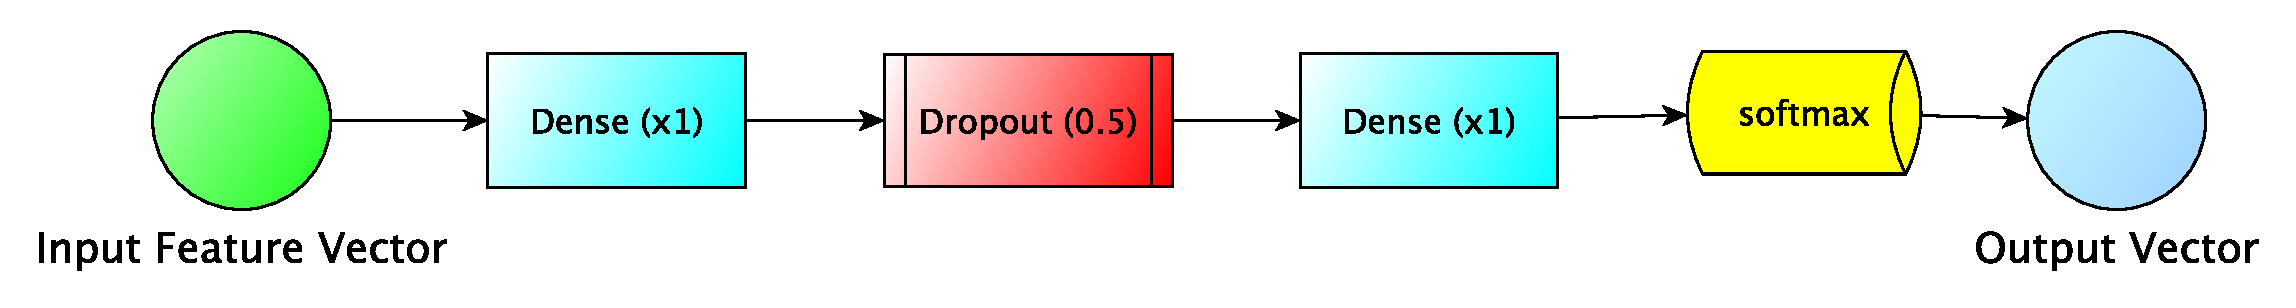
\includegraphics[width=0.85\textwidth]{figures/search_hh/mva/nn_arch_graph_updated}
        \caption{
            Illustration of the neural network graph employed in the analysis.
            The input feature vector has a length of 35 and the output vector is length 4,
            one for each of the targetted processes.
        }
        \label{fig:nn_arch}
    \end{center}
\end{figure}
Each of the dense layers are 250 nodes wide and  have their weights randomly initialized by sampling
from a truncated normal distribution centered on zero with a width given by $\sqrt{1/N_{\text{inputs}}}$, where
$N_{\text{inputs}}$ is the number of input features (the length of the input vector).
The activation functions for each of the dense layers are rectified linear units (`ReLu')~\cite{ReLu}.

Using an output layer with a softmax activation function allows one to interpret the outputs as
each representing a probability\footnote{The use of the term `probability' here is only
loosely correct, as the outputs are not \textit{strictly} probabilities.}
for the output's associated class ($hh$, Top, $Z \rightarrow \{ee,\mu\mu\}$,
or $Z \rightarrow \tau\tau$) given the inputs and for this reason it is commonly used for multi-class
neural network classifiers.
The association of the softmax activation with a class probability can be seen by its definition,
\begin{align}
    a_j = \frac{ e^{z_j} } { \sum\limits_k e ^{z_k} },
    \label{eq:softmax_activation}
\end{align}
where $a_j$ is the activation of the $j^{th}$ output neuron, the $z_i$ are the inputs to the output layer,
and $k$ runs over all output neurons.
It can be seen that if one sums over all outputs of a layer whose activation is given by Equation~\ref{eq:softmax_activation}
that the sum is equal to one.
Thus, the outputs of the softmax layer can be seen as a probability distribution.
For this reason, in the discussion to follow, we refer to the outputs of our neural network as `$p_i$',
where $i$ has four possibiities for each of the four outputs: $i \in \{ hh, \text{Top}, Z\rightarrow ee/\mu\mu, Z\rightarrow \tau\tau \}$.

The use of droput layers during the training process of is a form of statistical learning regularization that is reminiscient
of ensemble methods in the non-deep-learning arena, such as random forests~\cite{RandomForestsBreiman2001}.
They act to randomly disable a tunable fraction of inputs during various points in the training stage~\cite{JMLRDropout}.
This tunable fraction is referred to as the \textit{dropout rate}.
The use of dropout regularization prevents nodes within the network from co-adapting too much, thus reducing
the effects of overtraining.
This is illustrated in Figure~\ref{fig:dropout_illustration}.
During each batch of events forwarded to the network during the training phase, the dropout layer disables
portions of the network and thereby presents a modified network to the inputs.
Conceptually, then, using dropout during training is similar to training a set of very many, different \textit{weak}
neural networks.
During test time, at the time when the neural network is actually being used in the analysis,
the network's weights, which have been determined after training over the set of thinned networks,
are scaled down by the dropout rate.
This is illustrated in Figure~\ref{fig:dropout_weight_scaling}.

\begin{figure}[!htb]
    \begin{center}
        \includegraphics[width=0.85\textwidth]{figures/search_hh/mva/dropout_illustration}
        \caption{
            Illustration of dropout regularization. Figure taken from Ref.~\cite{JMLRDropout}.
            \textit{\textbf{Left}}: A standard neural network with two fully-connected layers.
            \textit{\textbf{Right}}: An example of a thinned network produced by applying dropout to the
                network on the left.
                The units with `X' have been dropped.
        }
        \label{fig:dropout_illustration}
    \end{center}
\end{figure}

\begin{figure}[!htb]
    \begin{center}
        \includegraphics[width=0.85\textwidth]{figures/search_hh/mva/dropout_weight_scaling}
        \caption{
            Illustration of the dropout rate effect on the network weights. Figure taken from Ref.~\cite{JMLRDropout}.
            \textit{\textbf{Left}}: A node in a fully-connected layer at training time is present in the network with
                a probability equal to the dropout rate and is connected to the next layer with weights represented by $\bm{w}$.
            \textit{\textbf{Right}}: At test time, the node is present with 100\% probability but its weights are scaled down by the
                dropout rate, $p\bm{w}$.
        }
        \label{fig:dropout_weight_scaling}
    \end{center}
\end{figure}

\noindent
As mentioned above, the use of dropout regularization prevents nodes within the network from co-adapting
too much and forces the network to learn more robust features that are useful in conjunction with many 
different random subsets of the other nodes.
That is, dropout regularization ensures that the model is robust against the loss of any individual
``piece of evidence'' and is found to reduce the effects of overtraining, which improves the generalizability
of the trained classifier.

The neural network classifier used in the present analysis, illustrated in Figure~\ref{fig:nn_arch},
uses a single dropout layer acting on the first fully-connected node and is given a dropout rate of 50\%.

During training, the loss metric is the categorical crossentropy and the Adam optimization algorithm~\cite{AdamOptimizer} is used.\footnote{More
on categorical cross-entropy: \href{https://ml-cheatsheet.readthedocs.io/en/latest/loss_functions.html\#cross-entropy}
{https://ml-cheatsheet.readthedocs.io/en/latest/loss\_functions.html\#cross-entropy}}


%%%%%%%%%%%%%%%%%%%%%%%%%%%%%%%%%%%%%%%%%%%%%%%%%%%%%%%%%%%%%%%%%%%%%%%%%%%%%%%%%%%
%%%%%%%%%%%%%%%%%%%%%%%%%%%%%%%%%%%%%%%%%%%%%%%%%%%%%%%%%%%%%%%%%%%%%%%%%%%%%%%%%%%
%%%%%%%%%%%%%%%%%%%%%%%%%%%%%%%%%%%%%%%%%%%%%%%%%%%%%%%%%%%%%%%%%%%%%%%%%%%%%%%%%%%
%
% TRAINING AND ARCHITECTURE
%
%%%%%%%%%%%%%%%%%%%%%%%%%%%%%%%%%%%%%%%%%%%%%%%%%%%%%%%%%%%%%%%%%%%%%%%%%%%%%%%%%%%
%%%%%%%%%%%%%%%%%%%%%%%%%%%%%%%%%%%%%%%%%%%%%%%%%%%%%%%%%%%%%%%%%%%%%%%%%%%%%%%%%%%
%%%%%%%%%%%%%%%%%%%%%%%%%%%%%%%%%%%%%%%%%%%%%%%%%%%%%%%%%%%%%%%%%%%%%%%%%%%%%%%%%%%
